\documentclass{article}
\usepackage{amsmath}
\usepackage{graphicx}
\usepackage[utf8]{inputenc}
\usepackage[T1, T2A]{fontenc}
\usepackage[english,russian]{babel}

\title{Задачи к теорминимуму}
\author{Anikin Evgeny, 121}

\begin{document}
\maketitle
	\section{Задача про колесо}
	\subsection{Ответ}
	Колесо не проскальзывает, если выполняется неравенство
	\begin{equation}
		k > \frac{\epsilon}{3} 
			\frac{|2gR - v_0^2|}{\sqrt{(gR)^2 - (2\epsilon v_0^2)^2}} + O(\epsilon^2),
	\end{equation}
	\begin{equation}
		v_0^2 = \frac{2(E - mgR)}{m + I/R^2}
	\end{equation}	
	Потенциальная энергия отсчитывается от уровня пола.
	Область, где колесо проскальзывает (в первом порядке), закрашена на рисунке красным.
	\begin{figure}[ht]
		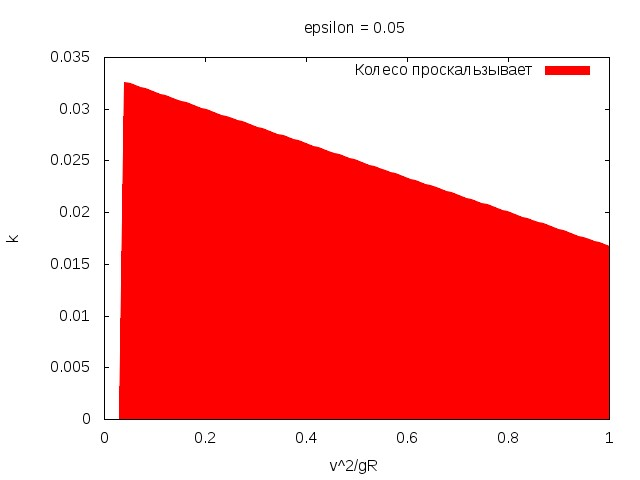
\includegraphics[width=\linewidth]{wheel.jpg}
	\end{figure}
	При $v_0^2 = 2gR$ минимальный коэффициент трения в первом порядке равен нулю.
	Во втором порядке он равен
	\begin{equation}
		k_{\mathrm{min}} = \frac{5}{6}\epsilon^2
	\end{equation}
	Это будет означать, что граница красной области на рисунке не будет подходить к оси абсцисс
	при $v_0^2 = 2gR$, а будет просто иметь минимум.

	Область допустимых значений параметра $v_0$ такова: $v_0^2 > 2gR\epsilon/3$ (это берётся из
	условия, что колесо движется поступательно, а не колеблется).
	\subsection{Решение}
	Примем следующие обозначения: пусть $R(1 + \epsilon/2)$, 
	$R(1 - \epsilon/2)$ --- полуоси эллиптического колеса,
	$\alpha$ --- угол поворота, $x$, $y$ --- координаты центра масс колеса, $\xi$ --- смещение
	центра масс относительно точки касания по горизонтали (см. рисунок). 
	\begin{figure}[h]
		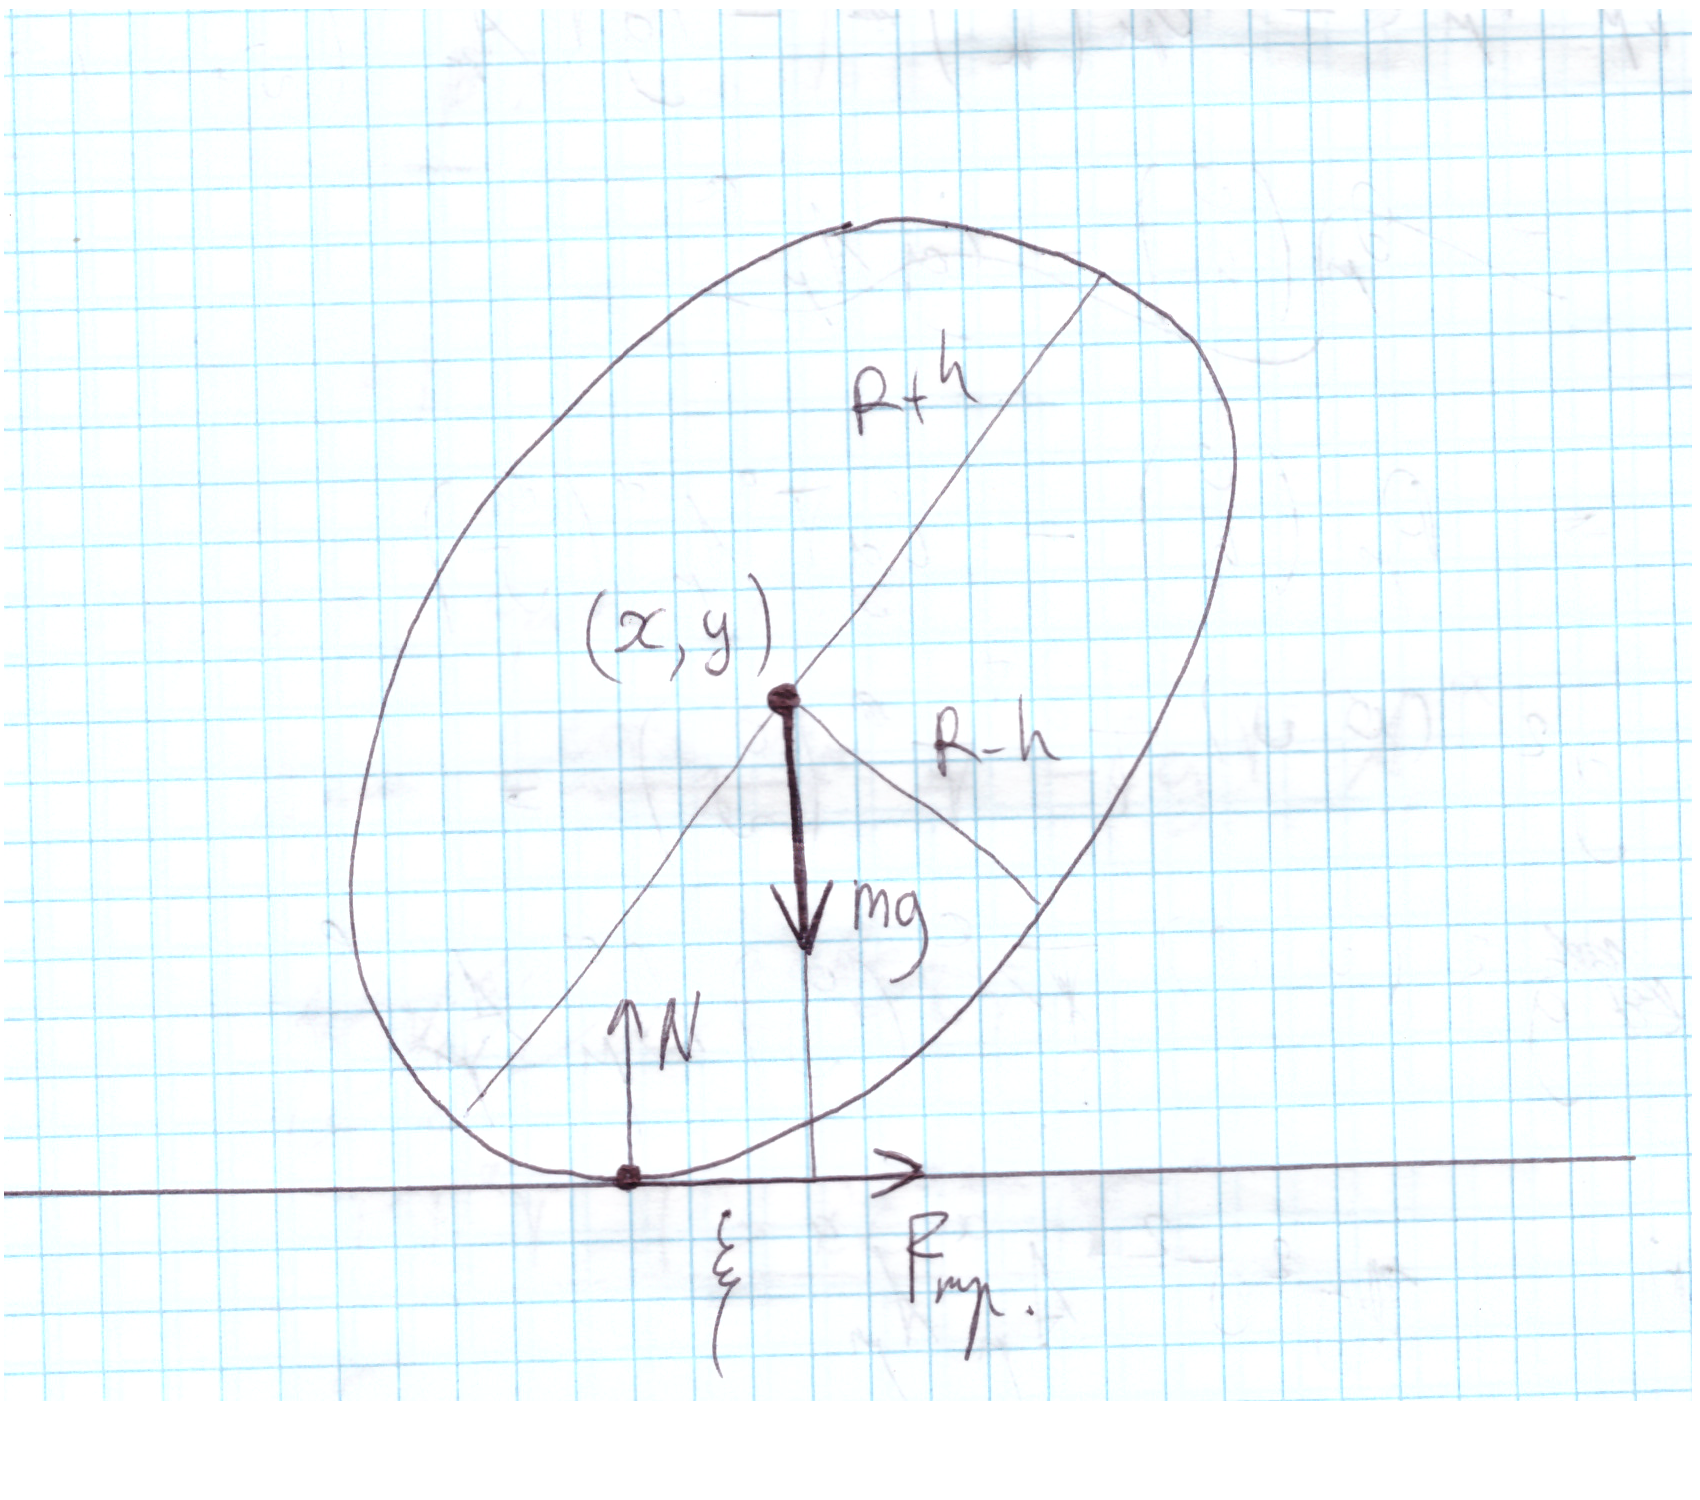
\includegraphics[width=\linewidth]{ellipsis.png}
	\end{figure}
	
	Очевидны следующие формулы (точные)
	\begin{equation}
		\label{eq1}
		x' = y
	\end{equation}
	\begin{equation}
		\label{eq2}
		x'' = y' = -\xi
	\end{equation}

	Ещё в первом порядке по $\epsilon$ верны равенства:	
	\begin{equation}
		\label{rad}
		y(\alpha) = R\left(1 + \frac{\epsilon}{2} \cos{2\alpha} + O(\epsilon^2) \right )
	\end{equation}
	\begin{equation}
		\label{xi}
		\xi(\alpha) = R\left(\epsilon\sin{2\alpha} + O(\epsilon^2)\right)
	\end{equation}

	Теперь напишем законы Ньютона для колеса.
	\begin{equation}
		I\dot{\omega} = N\xi - F_{\mathrm{tr}}y
	\end{equation}
	\begin{equation}
		m\ddot{x} = F_{\mathrm{tr}}
	\end{equation}
	\begin{equation}
		m\ddot{y} = -mg + N
	\end{equation}
	Исключая силы трения и реакции опоры, получим уравнение
	\begin{equation}
		I\dot{\omega} = m(\ddot{y} + g)\xi - m\ddot{x}y
	\end{equation}
	Используя очевидные равенства $\ddot{x} = x''\omega^2 + x'\dot{\omega}$, 
	$\ddot{y} = y''\omega^2 + y'\dot{\omega}$ (штрихи означают
	производную по углу $\alpha$), можно выразить угловое ускорение через
	угловую скорость и угол.
	\begin{equation}	
		\label{ddotomega}
		\dot{\omega} = \frac{(y''\xi - x''y)\omega^2 + g  }{ I/m - y'\xi + x'y }
	\end{equation}
	или, используя \ref{eq1}, \ref{eq2},
	\begin{equation}
		\dot{\omega} = \xi\,\frac{(y - \xi')\omega^2 + g}{I/m + y^2 + \xi^2}
	\end{equation}
	
	Отсюда следует точное выражение для $\ddot{x}$.
	\begin{equation}
		\ddot{x} = \frac{g\xi y}{I/m + y^2 + \xi^2} - \xi \omega^2
						\, \frac{y\xi' + \xi^2 + I/m}{I/m + y^2 + \xi^2}
	\end{equation}
	Пользуясь законом сохранения энергии,
	\begin{equation}
		E = \frac{I\omega^2}{2} + \frac{m(y^2 + \xi^2)\omega^2}{2} + mgy
	\end{equation}
	\begin{equation}
		\omega^2 = \frac{2(E/m - gy)}{I/m + y^2 + \xi^2}
	\end{equation}
	перепишем выражение для $\ddot{x}$.
	
	\begin{equation}
		\label{ddotx}
		\ddot{x} = x''\omega^2 + x'\dot{\omega} =  \xi\left [\frac{gy}{I/m + y^2 + \xi^2} 
						- \frac{2(E/m - gy)(y\xi' + \xi^2 + I/m)}
									{(I/m + y^2 + \xi^2)^2} \right ]
	\end{equation}
	Пусть дальше $\lambda = 0.5$, $I = \lambda mR^2$, 
	$E = mgR + \frac{(\lambda+1)mv_0^2}{2}$. ($v_0$ здесь --- не 
	скорость, а просто параметр).
	В первом порядке по $\epsilon$
	\begin{equation}
		\ddot{x} = \epsilon\sin{2\alpha}\frac{gR - \lambda v_0^2}{(\lambda + 1)R}
	\end{equation}
	То же самое можно сделать для $\ddot{y}$, но точное выражение нам не понадобится. В первом 
	порядке по $\epsilon$ 
	\begin{equation}
		\ddot{y} = -\xi'\omega^2 = -2\epsilon\frac{v_0^2}{R}\cos{2\alpha}
	\end{equation}
	
	Условие того, что колесо не проскальзывает, можно записать так:
	\begin{equation}
		\label{ineq}
		k > \left|\frac{\ddot{x}}{\ddot{y} + g}\right| = 
		\left| \frac{2gR - v_0^2}{3}
		\frac{\epsilon\sin{2\alpha}}{gR - 2\epsilon v_0^2\cos{2\alpha}}\right|
	\end{equation}
	Нужно найти угол, при котором выражение 
	в правой части предыдущего равенства максимально.
	Дифференцируя правую часть, приходим к условию
	\begin{equation}
		\cos{2\alpha} = \frac{2\epsilon v_0^2}{gR}
	\end{equation}
	Подставляя в \ref{ineq}, получим
	\begin{equation}
		k > \frac{\epsilon}{3} 
			\frac{2gR - v_0^2}{\sqrt{(gR)^2 - (2\epsilon v_0^2)^2}}
	\end{equation}

	При $v_0^2 = 2gR$ сила трения обращается в нуль в первом порядке по $\epsilon$.
	Поэтому минимальный коэффициент трения тоже равен нулю в первом порядке.
	
	При $v_0^2 = \frac{gR}{2\epsilon}$ обращается в нуль сила реакции опоры. Это значит, что 
	колесо начнёт подпрыгивать.
	
	Если $v_0^2 \gg gR\epsilon$, то $v_0$ равно скорости движения колеса с точностью
	до членов порядка $\epsilon$. 

	Найдём минимальный коэффициент трения при $v^2 = 2gR$ во втором порядке.
	Для этого нужно разложить \ref{ddotx} до следующего порядка. Так как при $v^2 = 2gR$ 
	выражение в квадратных скобках в формуле \ref{ddotx} обращается в нуль в нулевом порядке,
	нужно разложить до первого порядка выражение в квадратных скобках,
	а $\xi$ во втором порядке 	искать не нужно. 
	
	После неинтересных выкладок (раскладываем часть \ref{ddotx} в квадратных скобках 
	до первого порядка, подставляем значение $v_0$ и значение $\xi$ в первом порядке) 
	получается такой ответ:
	\begin{equation}
		\ddot{x} = -\frac{5}{6} g\epsilon^2 \sin{4\alpha}
	\end{equation}
	Так как $v^2 = 2gR \ll \frac{gR}{2\epsilon}$, можно не учитывать изменения $\ddot{y}$.
	Поэтому минимальный коэффициент трения ---
	\begin{equation}
		k_{\mathrm{min}} = \frac{5}{6}\epsilon^2
	\end{equation}
		
\end{document}
